%--------------------------------------------------------------------------------------
% Este arquivo contém a sua introdução, objetivos e organização do trabalho
%--------------------------------------------------------------------------------------
\chapter{Introdução} \label{ch:Introdução}
    A informatização do mundo, juntamente com a evolução dos equipamentos computacionais, vem permitindo a geração e coleta de enormes volumes de dados das mais variadas fontes, podendo-se afirmar que vivemos na era dos dados \cite[p.~1]{Han:2011:DMC:1972541}.
    Grande parte dos dados criados \textit{online} está em forma de texto (escrito em linguagem natural) e um estudo feito pela Universidade da Califórnia em Berkeley em 2003 apontou, por exemplo, que somente notícias de jornais (considerando armazenamento digital do texto dos mesmos) representavam cerca de 13,5 terabytes por ano, livros cerca de 5,5 terabytes por ano, e e-mails mais de 440 exabytes por ano \cite{lyman2003much} \cite[p.~3]{Zhai2016TDMA}.
    
    A coleta e análise da sobrecarga diária de dados se apresenta como um problema que a Mineração de Texto tenta resolver no caso de dados textuais, utilizando de técnicas de mineração de dados, aprendizado de máquina, processamento de linguagem natural, Recuperação de Informação, e gerenciamento do conhecimento \cite[p.~1]{Han:2011:DMC:1972541} \cite{Feldman:2006:TMH:1076381}.
    Técnicas de Mineração de Texto são aplicadas na classificação e clusterização de documentos, sumarização de opiniões na internet, acesso de dados biomédicos \cite[p.~4--8]{Aggarwal_MTD_2012},
    e também em tarefas de identificação de perfis de autoria\footnotemark{} \cite[p.~906]{rangel2014overview} \cite[p.~6--7]{rangel2018overview}, auxiliando em investigações forenses linguísticas \cite{Chaski_Author_2012}. 
    
    \footnotetext{A identificação de perfis de autoria consiste na extração de características do autor com base no conteúdo e estilo do texto. Essas características podem ser gênero, faixa etária, escolaridade, entre outras \cite[p.~266]{WEREN_ARTIGO_2014}.}
    % A aplicação de técnicas de Mineração de Texto nos grandes volumes de dados
    %  e é portanto uma necessidade importante,
    
% Motivação
% Importância de MT, citar exemplos práticos (encontrar criminosos, forense ) CHECK
    % motivação informal
    % existe essa área, MT, que é útil para diversas tarefas, como por exemplo classificação de grandes volumes de texto, identificação de perfil de autor e tal.
    % ela utiliza de suporte a RI para fazer suas funções, e nas tarefas de classificação são indicados atributos do dados na representação, a engenharia de atributos permite então definir bons atributos para dados textuais
    % dentre os atributos, podem ser gerados atributos oriundos de funções de RI
    % na MT cada modelo de classificação sofre uma avaliação comparativa de desempenho, o uso de diferentes atributos impacta no desempenho do classificador
    % assim, encontrar um conjunto de atributos que melhore o desempenho de classificadores de MT é uma tarefa difícil
    % encontrar meios de melhorar o desempenho dos classificadres é um dos objetivos da MT, e utilizar novos conjuntos de atributos pode trazer avanços nesse sentido
    \begin{figure}[ht]
    \centering
    \caption{Tarefa de categorização de texto (com exemplos de treinamento disponíveis).}
    \begin{center}
        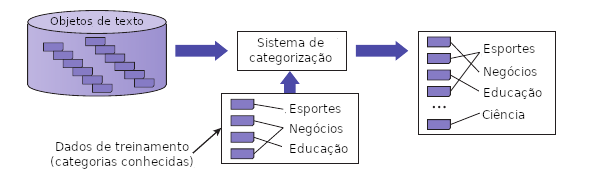
\includegraphics[width=0.75\textwidth]{img/figure15-1-zhai-traduzido.png}
    \end{center}
    \vspace{-0.5cm}
    \legend{\ABNTEXfontereduzida \textbf{Fonte:} Figura adaptada de \citeonline[p.~300]{Zhai2016TDMA}.}
    \label{fig:categorização-de-texto-zhai2016}
\end{figure}
    
    A Mineração de Texto aborda, dentre seus tipos de tarefas oriundas da mineração de dados, a tarefa de classificação nas coleções de documentos, geralmente chamada de classificação de texto ou categorização de texto \cite[p.~35]{Zhai2016TDMA}.
    Classificação é definido como o processo de designar uma, ou mais, categorias a cada objeto de texto, dentre categorias predefinidas, sendo que predominantemente é utilizado um conjunto de textos já classificado para treinamento \cite[p.~7]{Jo2018TMCIBDC} \cite[p.~299]{Zhai2016TDMA}, esse processo está exemplificado na Figura \ref{fig:categorização-de-texto-zhai2016}.
    
    No processo de classificação de texto são derivados atributos dos objetos de texto originais, um passo necessário para funcionamento do modelo de classificação originário do aprendizado de máquina.
    Diferentes conjuntos de atributos podem impactar diretamente no desempenho de um classificador \cite[p.~304--306]{Zhai2016TDMA}, o qual é tipicamente mensurado pela acurácia\footnotemark{} \cite[p.~313--314]{Zhai2016TDMA} \cite[p.~9]{Jo2018TMCIBDC}.
    
    \footnotetext{Número de previsões corretas dividido pelo número total de previsões feitas \cite[p.~313]{Zhai2016TDMA}.}
    
    A sugestão de parâmetros
    
    Dentre as métricas para 
    
    
    A Mineração de Texto utiliza de diversas técnicas desenvolvidas pela área de Recuperação de Informação no seu processamento de texto
    
    Sistemas de RI são feitos para armazenar documentos e permitirem a sua consulta por usuários, 

% Definição do Problema
% Complexidade de RI na MT.	Dizer que RI é uma área, e vamos buscar ferramentas que subsidiam o cálculo das variáveis de RI. 


% Objetivo Geral
% Objetivo Especifico
% Organização do Trabalho
% \lipsum[5-10]

    \section{Justificativa} \label{sec:Justificativa}

% \lipsum[1]


    \section{Objetivos gerais} \label{sec:Objetivos-gerais}

% \lipsum[1]
% Avaliar o desempenho de técnicas de RI como atributos em MT
% Avaliar o desempenho de ferramentas computacionais para construção (indexação) de BDs e criação dos atributos de RI.
% Avaliar o desempenho dos classificadores de MT com e sem as var de RI.

    \section{Objetivos específicos} \label{sec:Objetivos-específicos}
    
    \begin{itemize}
    	\item x1;
        \item x2;
        \item x3.
    \end{itemize}
    
    \section{Organização do trabalho} \label{sec:Organização-do-trabalho}

% \lipsum[10-12]
